\documentclass[12pt]{amsart}

\addtolength{\hoffset}{-2.25cm}
\addtolength{\textwidth}{4.5cm}
\addtolength{\voffset}{-2.5cm}
\addtolength{\textheight}{5cm}
\setlength{\parskip}{0pt}
\setlength{\parindent}{15pt}

\usepackage[export]{adjustbox}
\usepackage{listings}
\usepackage{amsthm}
\usepackage{amsmath}
\usepackage{amssymb}
\usepackage[colorlinks = true, linkcolor = black, citecolor = black, final]{hyperref}

\usepackage{graphicx}
\usepackage{multicol}
\usepackage{ marvosym }
\usepackage{wasysym}
\usepackage{tikz}
\usetikzlibrary{patterns}

\newcommand{\ds}{\displaystyle}
\DeclareMathOperator{\sech}{sech}


\setlength{\parindent}{0in}

\pagestyle{empty}

\begin{document}

\thispagestyle{empty}

{\scshape COSC 525} \hfill {\scshape \large Project 1: Artificial Neural Network} \hfill {\scshape 2021-02-14}

\smallskip 

{University of Tennessee} \hfill { Su-Ann Chong}

\smallskip

\hrule

\bigskip
\section{Introduction}
% A short introduction to the problem 
In this project, a simple artificial neural network (ANN) library is implemented. The library is implemented in an object oriented manner with three different classes, namely \texttt{Neuron}, \texttt{FullyConnectedLayer} and \texttt{NeuralNetwork} to provide three levels of abstraction for an ANN: \\
% \bigskip

\begin{center}
A \texttt{NeuralNetwork} object consists of an array of \texttt{FullyConnectedLayer} objects. \\
Each \texttt{FullyConnectedLayer} object contains an array of \texttt{Neuron} objects.\\
\end{center} 

\bigskip

In each iteration, the library does a forward pass by calculating the output of the neural network and a weights update using gradient descent. 

\section{Assumptions/choices made}
\begin{itemize}
\item The bias of a neuron is treated with an extra input value of 1. Hence, user needs to make sure to add an extra input value of 1 in each input array. \\

\item Binary cross entropy loss function can only be used when the output value ranges from 0 to 1. Error may occur when activation function used (e.g. linear function) does not guarantee the output value to be between 0 and 1. \\

\item Currently, this library can support two activation functions (linear/logistic) and two loss functions (square error and binary cross entropy). 

\end{itemize}

\section{Problems/Issues}
Nothing to add.

\section{How to run the code}

You can run the code with examples using the following command:
\begin{lstlisting}[language=bash]
$ python project1_suann.py [example|and|xor]
\end{lstlisting}

You can choose to run either the class example problem, the AND problem or the XOR problem. 

% \bigskip
% Otherwise, you can import the library and feed the neural network using your own dataset. Please follow the guidelines and review the assumptions stated in Section 2.

\vfill 

\pagebreak

\section{Results}
\subsection{The class example problem} One step backpropagation 

% \begin{multicols}{2}
Number of hidden layer: 1 \\
Activation function: Sigmoid \\
Loss function: Squared error \\
Learning rate: 0.5 \\
Number of iteration: 1 \\

The weights after the 1-step update:\\
$ w_1 = 0.14978732, ~~~~~~ w_2 = 0.19957463, ~~~~~~ b_1 = 0.34574630$ \\
$ w_3 = 0.24975842, ~~~~~~ w_4 = 0.29951684, ~~~~~~ b_2 = 0.34516843$ \\
$ w_5 = 0.35895608, ~~~~~~ w_6 = 0.40870723, ~~~~~~ b_3 = 0.53075162$ \\
$ w_7 = 0.51181741, ~~~~~~ w_8 = 0.56188906, ~~~~~~ b_4 = 0.61993806$ \\

\begin{figure}[h]
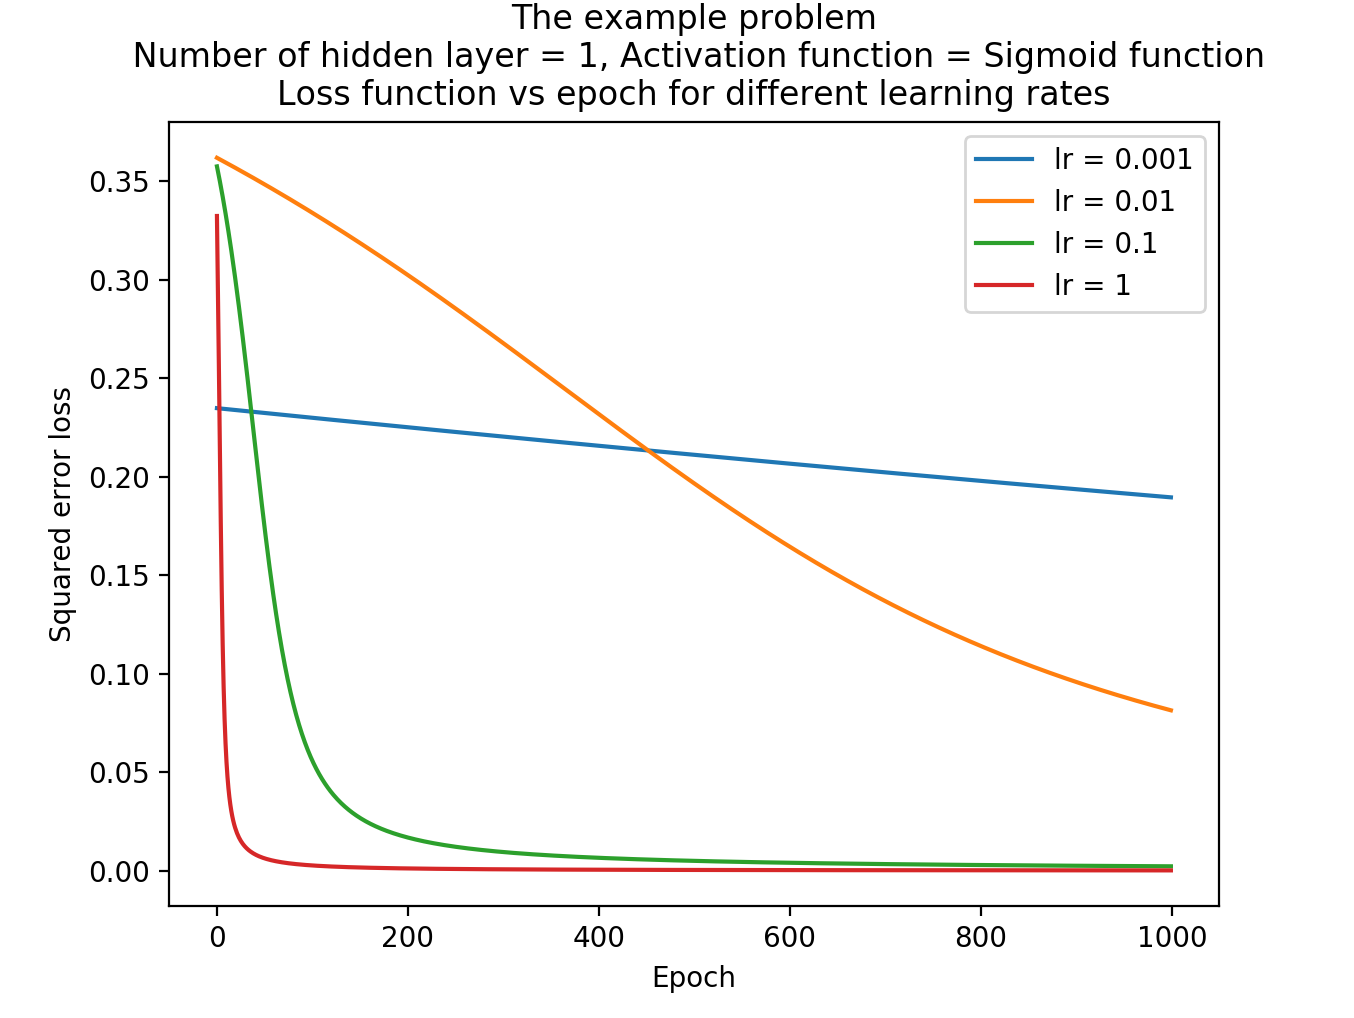
\includegraphics[width=0.49\columnwidth]{example_sigmoid_mse_lrs.png}
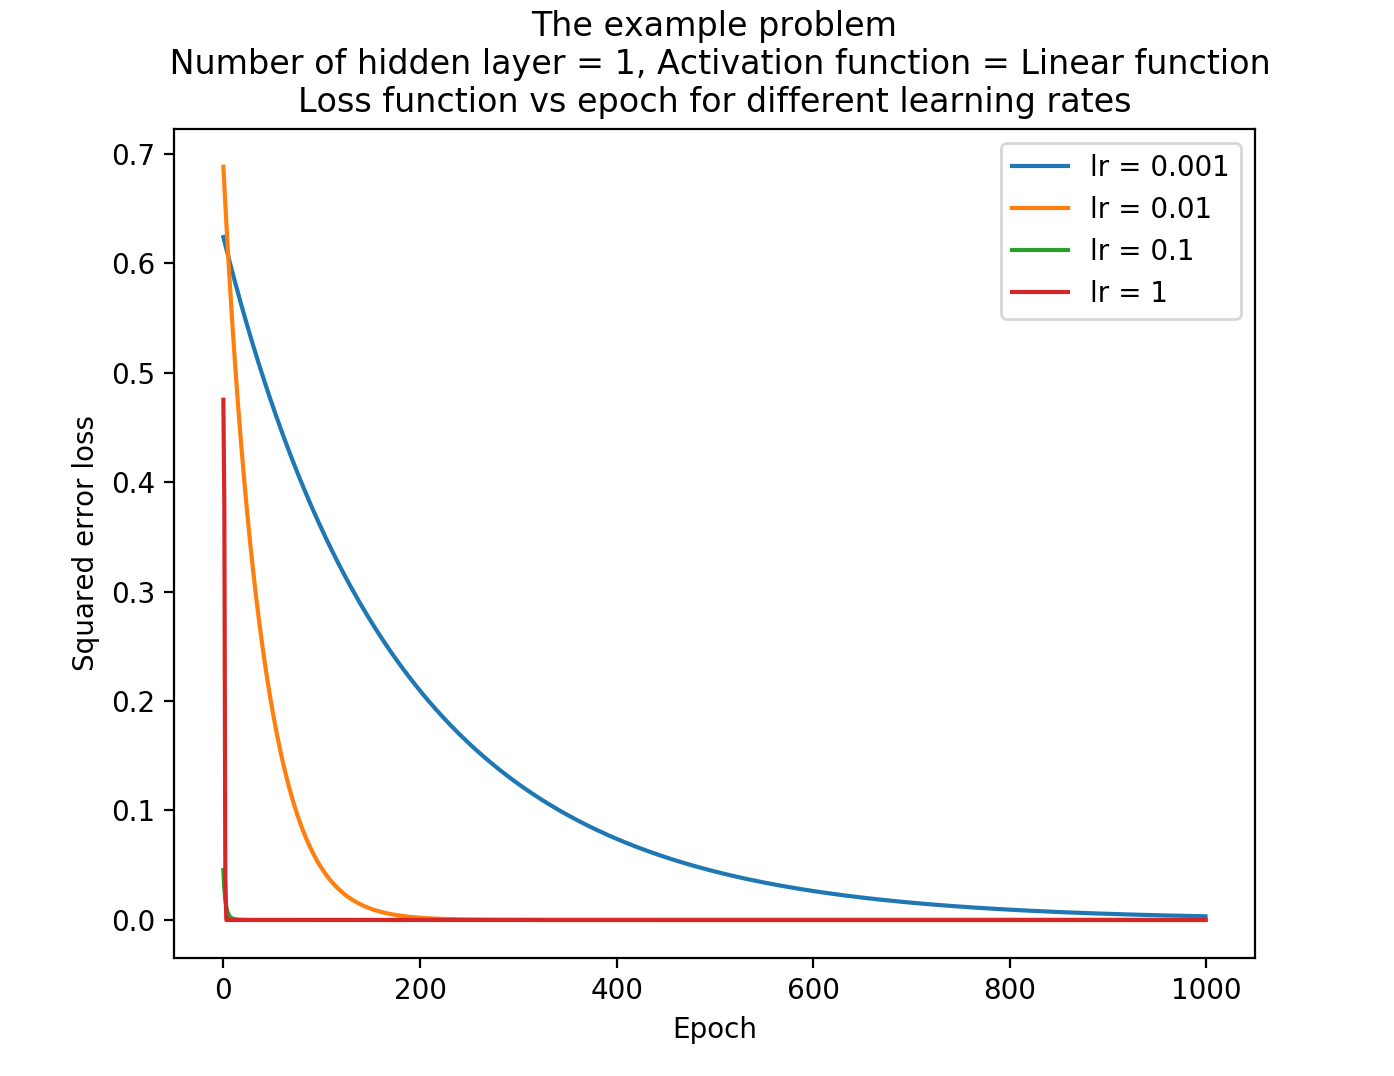
\includegraphics[width=0.49\columnwidth]{example_linear_mse_lrs.png}
\end{figure}

Using a sigmoid activation function, neural network with a larger learning rate converges faster with smaller loss as compared to a neural network with a smaller learning rate. \\

Using a linear activation function, the neural work seems to be able to converge very quickly and achieve small loss. Larger learning rate seems to converge faster and has smaller loss as compared to smaller learning rate.

\vfill

% \end{multicols}
\pagebreak
\subsection{The AND problem} A single perceptron\\
\begin{multicols}{2}
Number of hidden layer: 0 \\
Activation function: Sigmoid \\
Loss function: Squared error\\
Learning rate: 0.1
Number of iteration: 1000 \\
Predicted: $[[0.000], [0.055], [0.055], [0.935]] $ \\
Actual output: $[[0],[0],[0],[1]]$

Number of hidden layer: 0 \\
Activation function: Sigmoid \\
Loss function: Binary cross entropy\\
Learning rate: 0.1
Number of iteration: 1000 \\
Predicted: $[[0.000], [0.005], [0.005], [0.993]] $ \\
Actual output: $[[0],[0],[0],[1]]$
\end{multicols}

\begin{figure}[h]
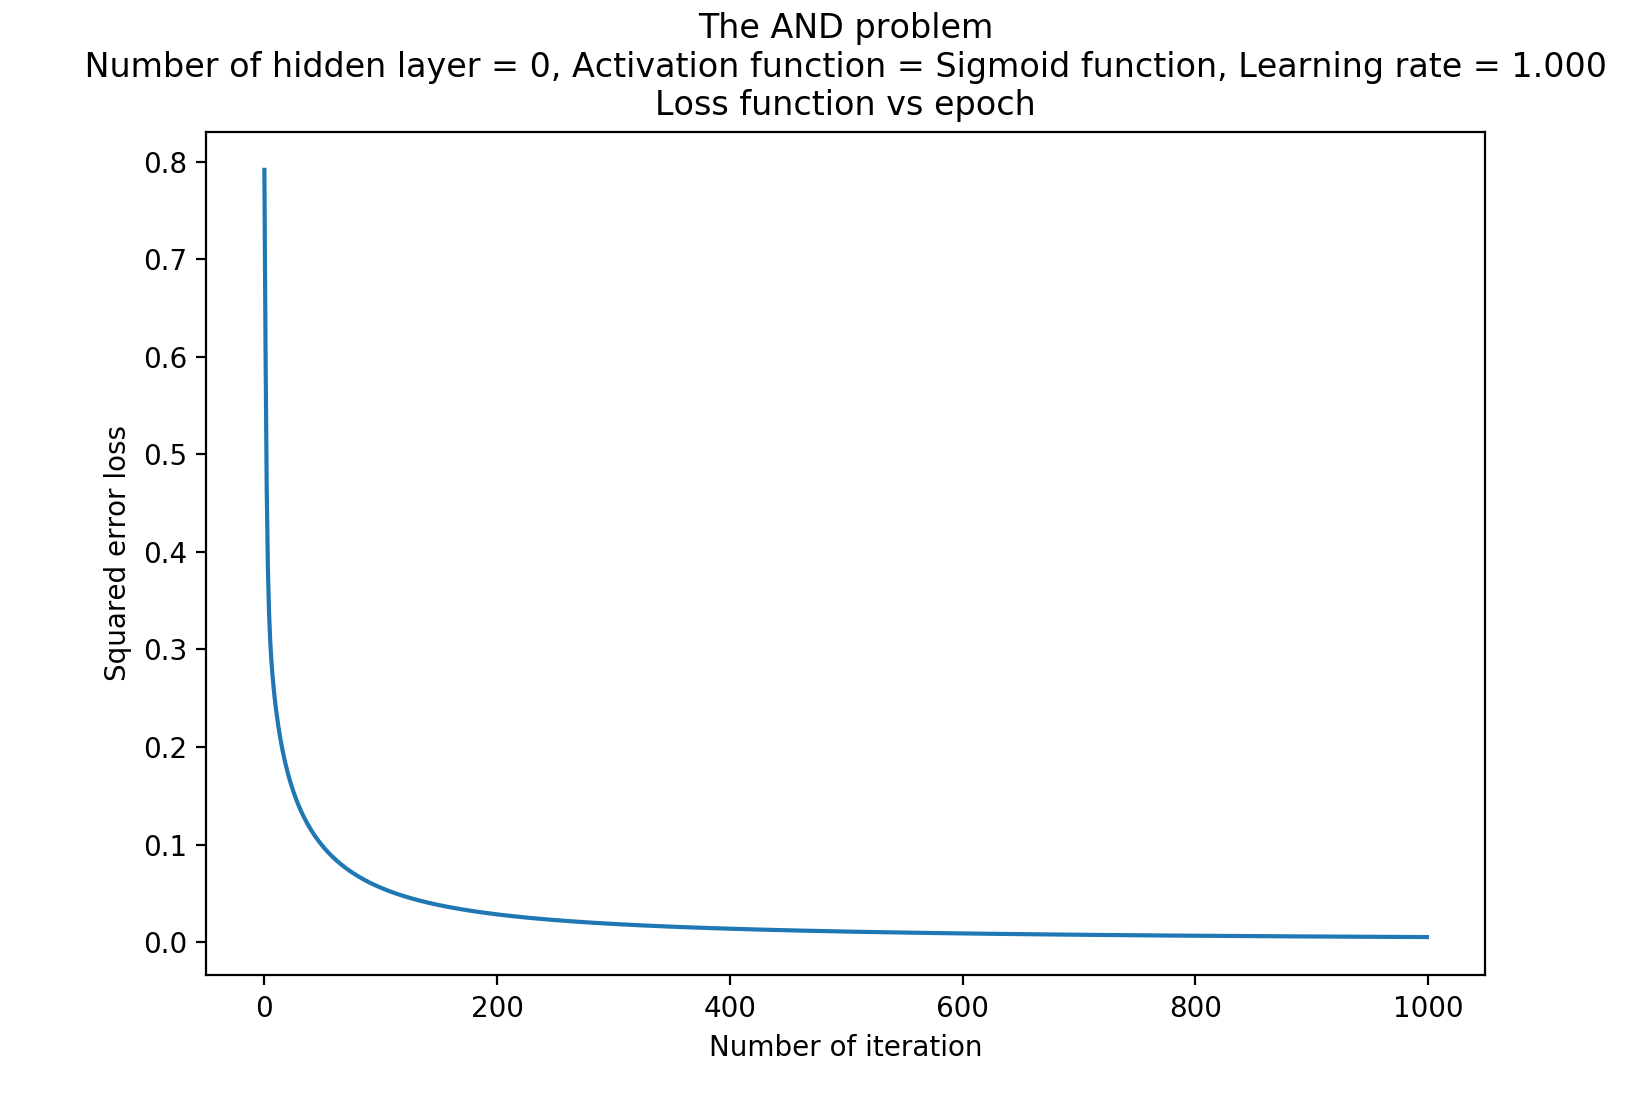
\includegraphics[width=0.49\columnwidth]{and_sigmoid_mse.png}
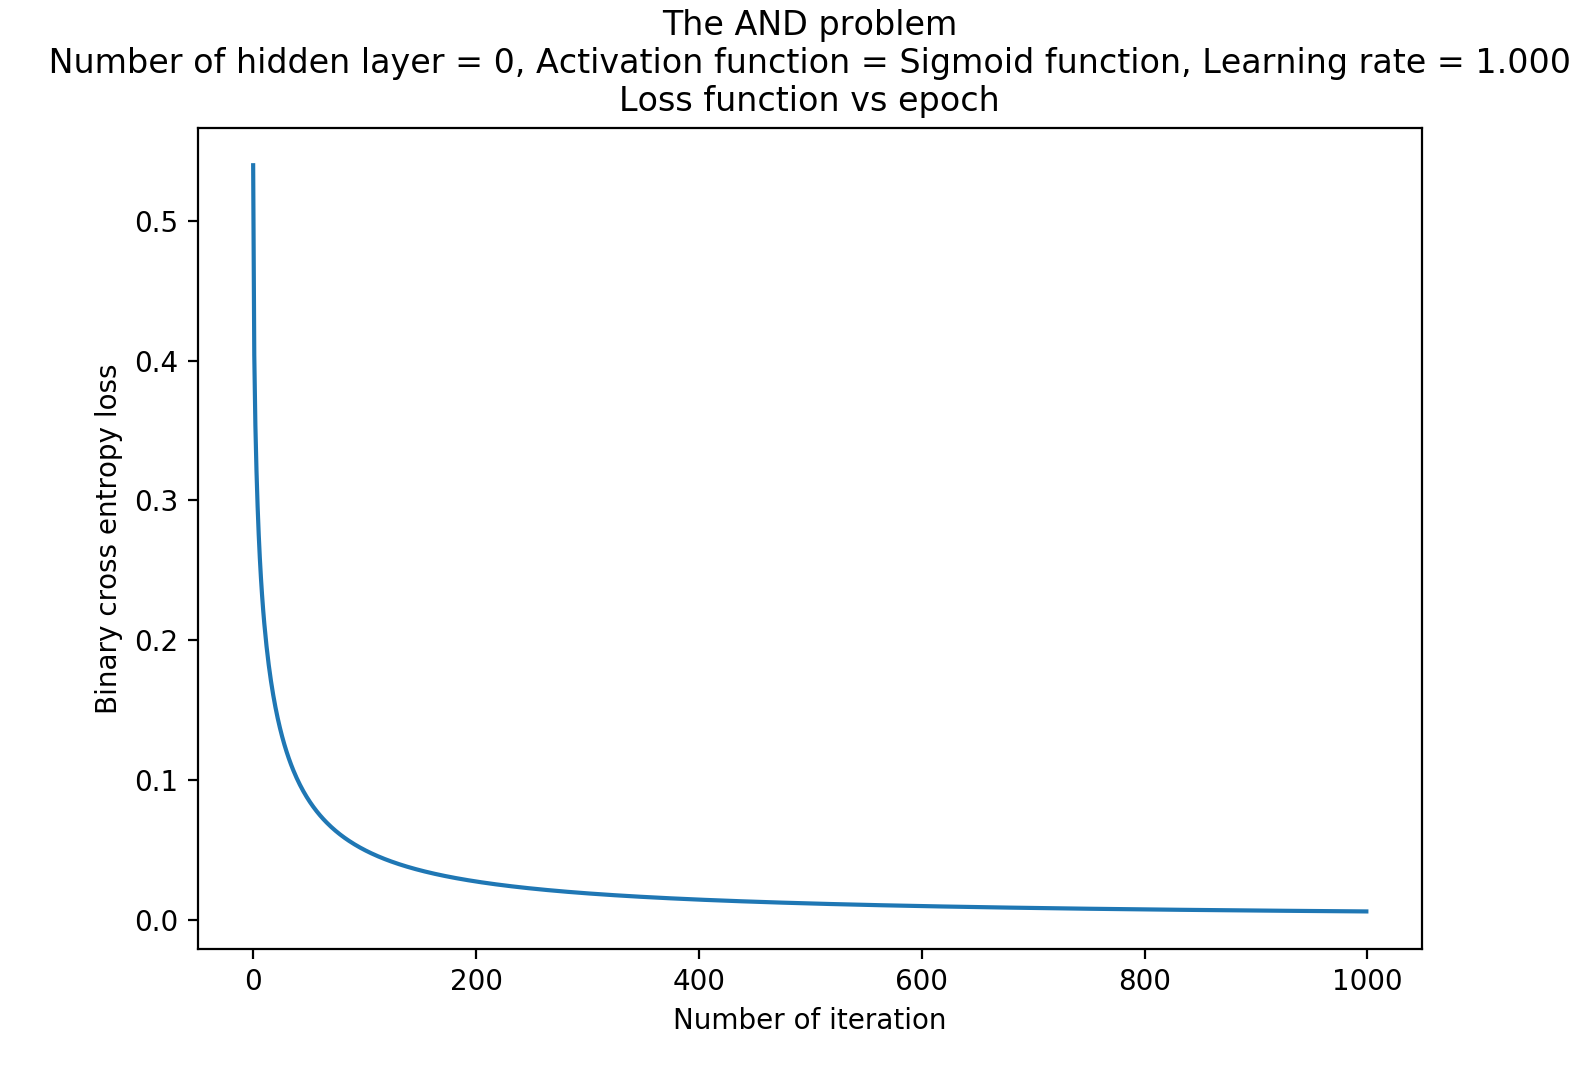
\includegraphics[width=0.49\columnwidth]{and_sigmoid_bce.png}
\end{figure}

A single perceptron (using sigmoid activation function) is able to solve the AND problem as it is a linear problem. \\

Number of hidden layer: 0 \\
Activation function: Linear \\
Loss function: Squared error \\
Learning rate: 0.01\\
Number of iteration: 1000 \\
Predicted: $[[-0.249], [0.248], [0.248], [0.755]] $ \\
Actual output: $[[0],[0],[0],[1]]$

\begin{figure}[h]
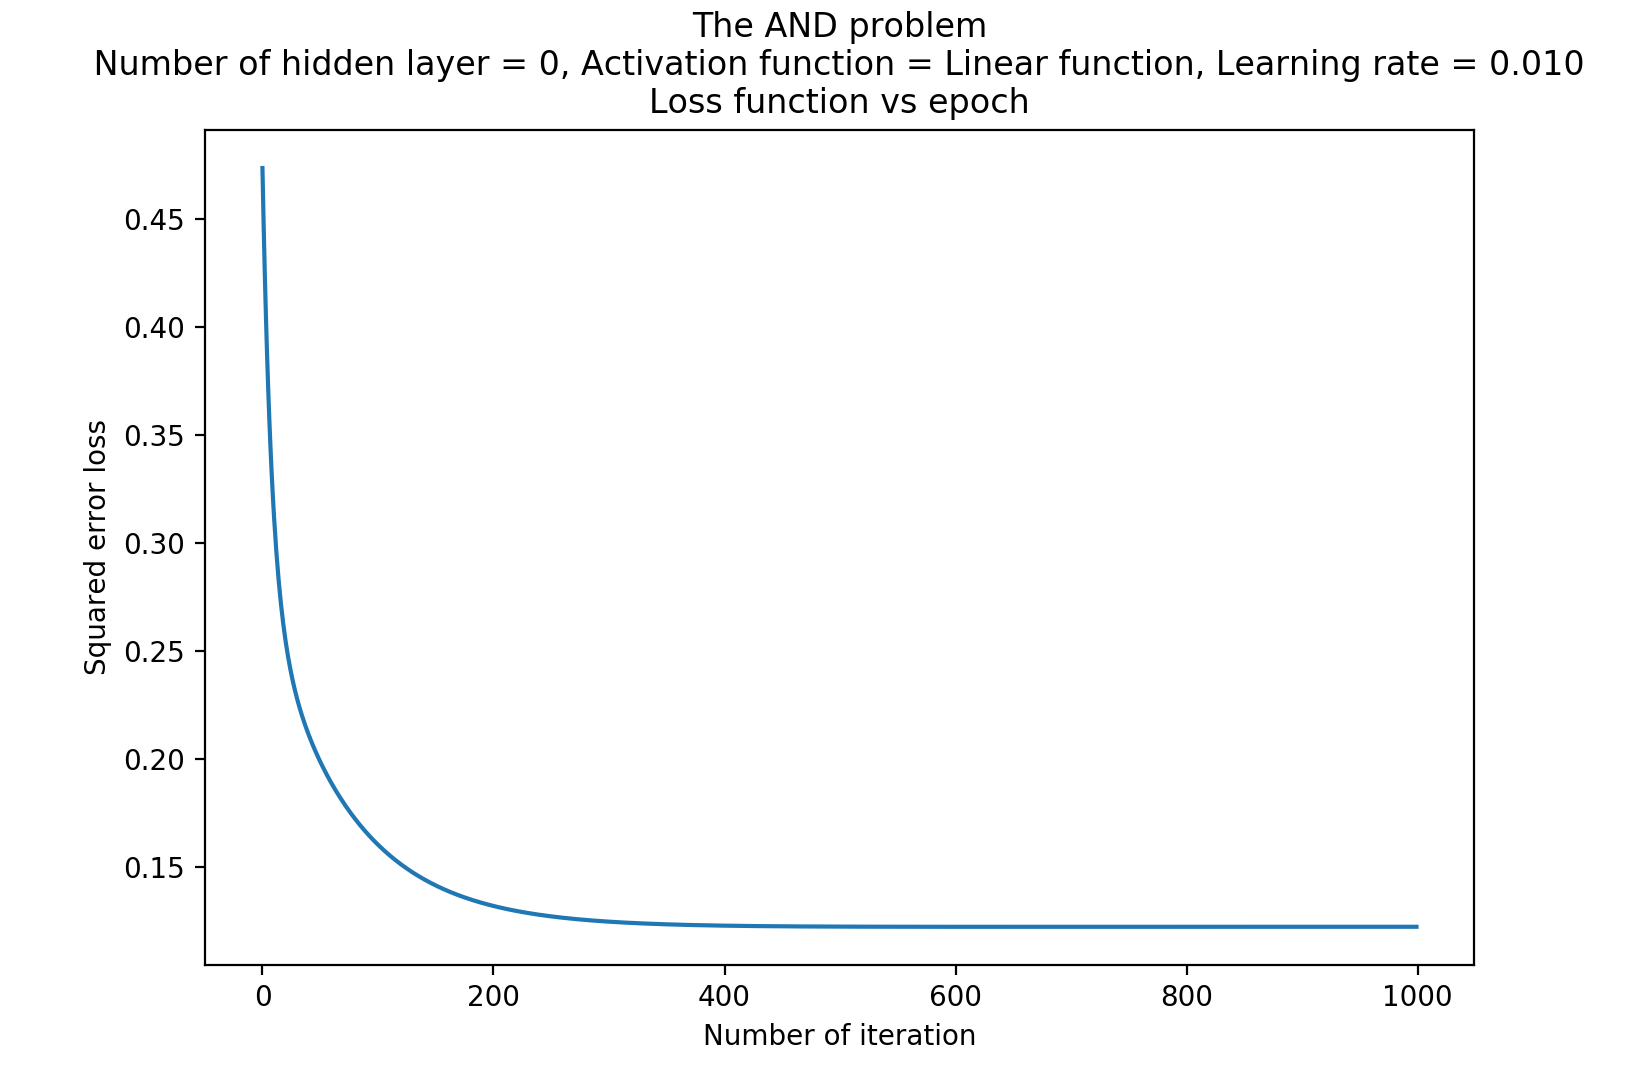
\includegraphics[width=0.49\columnwidth, left]{and_linear_mse.png}
\end{figure}

Using a linear function on a neural network without any hidden layer showed convergence in the solution, but the predicted output is far from the actual output. Only squared error is used because the predicted output consists of negative values. Binary cross entropy can only handle values range from 0 to 1. \\

\vfill
\pagebreak
\textbf{Single perceptron: loss functions vs epoch for different learning rates}

\begin{figure}[h]
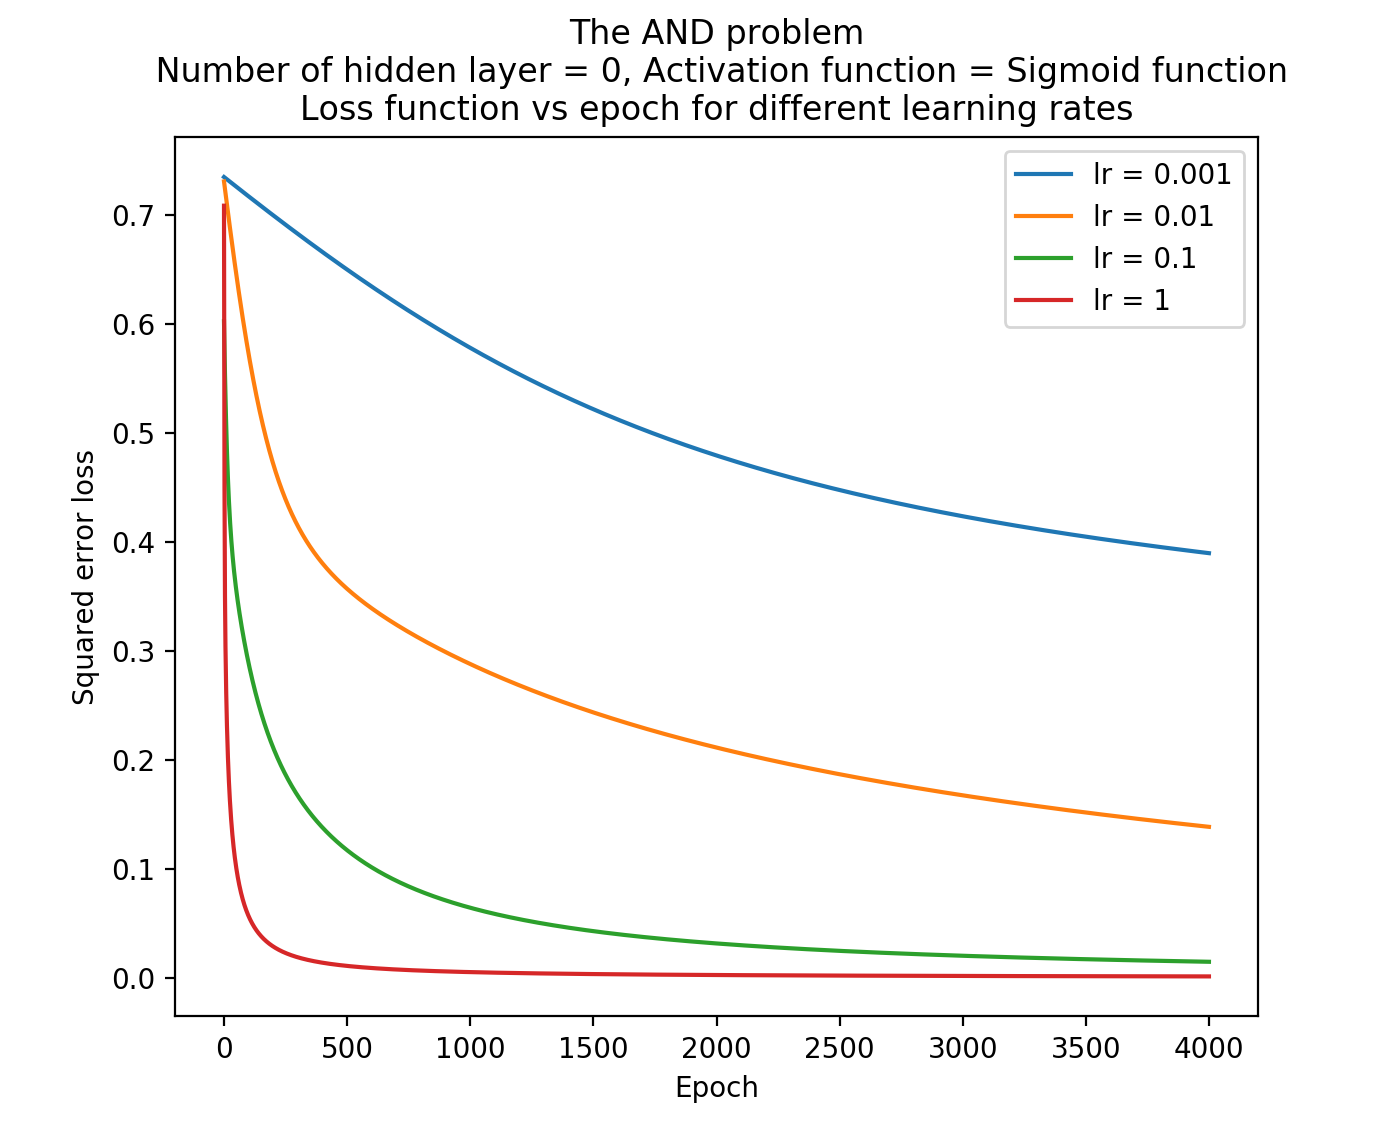
\includegraphics[width=0.49\columnwidth]{and_sigmoid_mse_lrs.png}
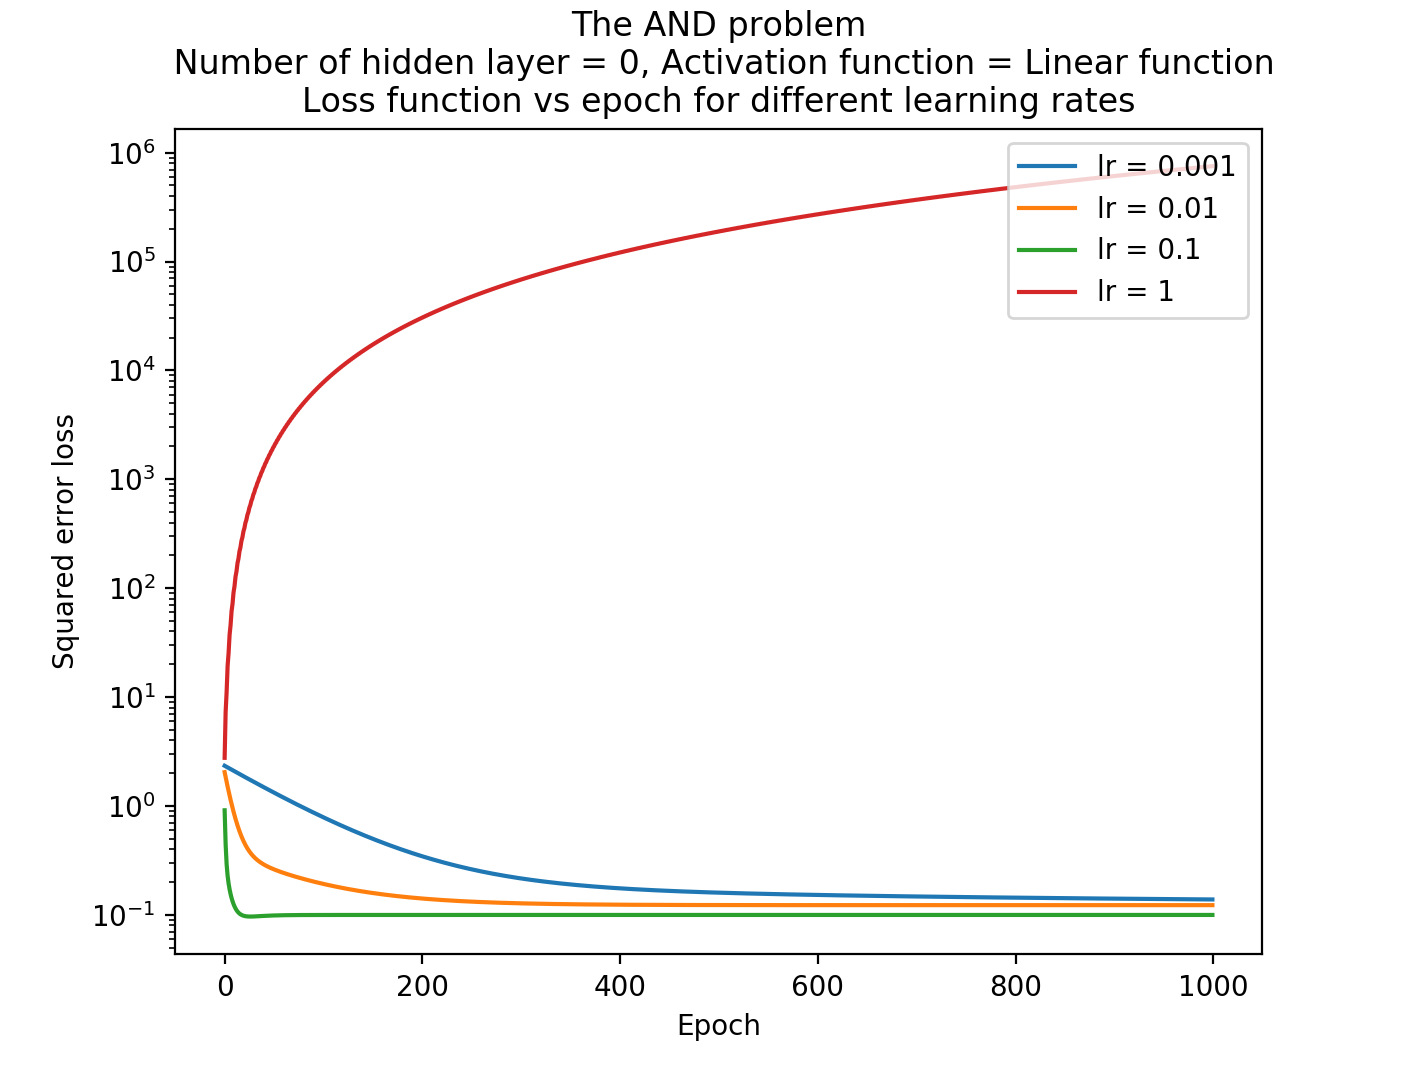
\includegraphics[width=0.49\columnwidth]{and_linear_mse_lrs.png}
\end{figure}

For sigmoid activation function, a larger learning rate seems to converge faster and has a lower loss. For linear activation function, too large of a learning rate results in an increasing loss. \\

% \pagebreak 
\subsection{The XOR problem} single perceptron and one hidden layer NN \\
\begin{multicols}{2}
Number of hidden layer: 0 \\
Activation function: Sigmoid \\
Loss function: Squared error\\
Learning rate: 0.01\\
Number of iteration: 1000 \\
Predicted: $[[0.480], [0.501], [0.494], [0.513]]$ \\
Actual output: $[[0],[1],[1],[0]]$

Number of hidden layer: 0 \\
Activation function: Linear \\
Loss function: Squared error\\
Learning rate: 0.001 \\
Number of iteration: 1000 \\
Predicted: $[[0.484], [0.490], [0.506], [0.510]]$ \\
Actual output: $[[0],[1],[1],[0]]$
\end{multicols}

\begin{figure}[h]
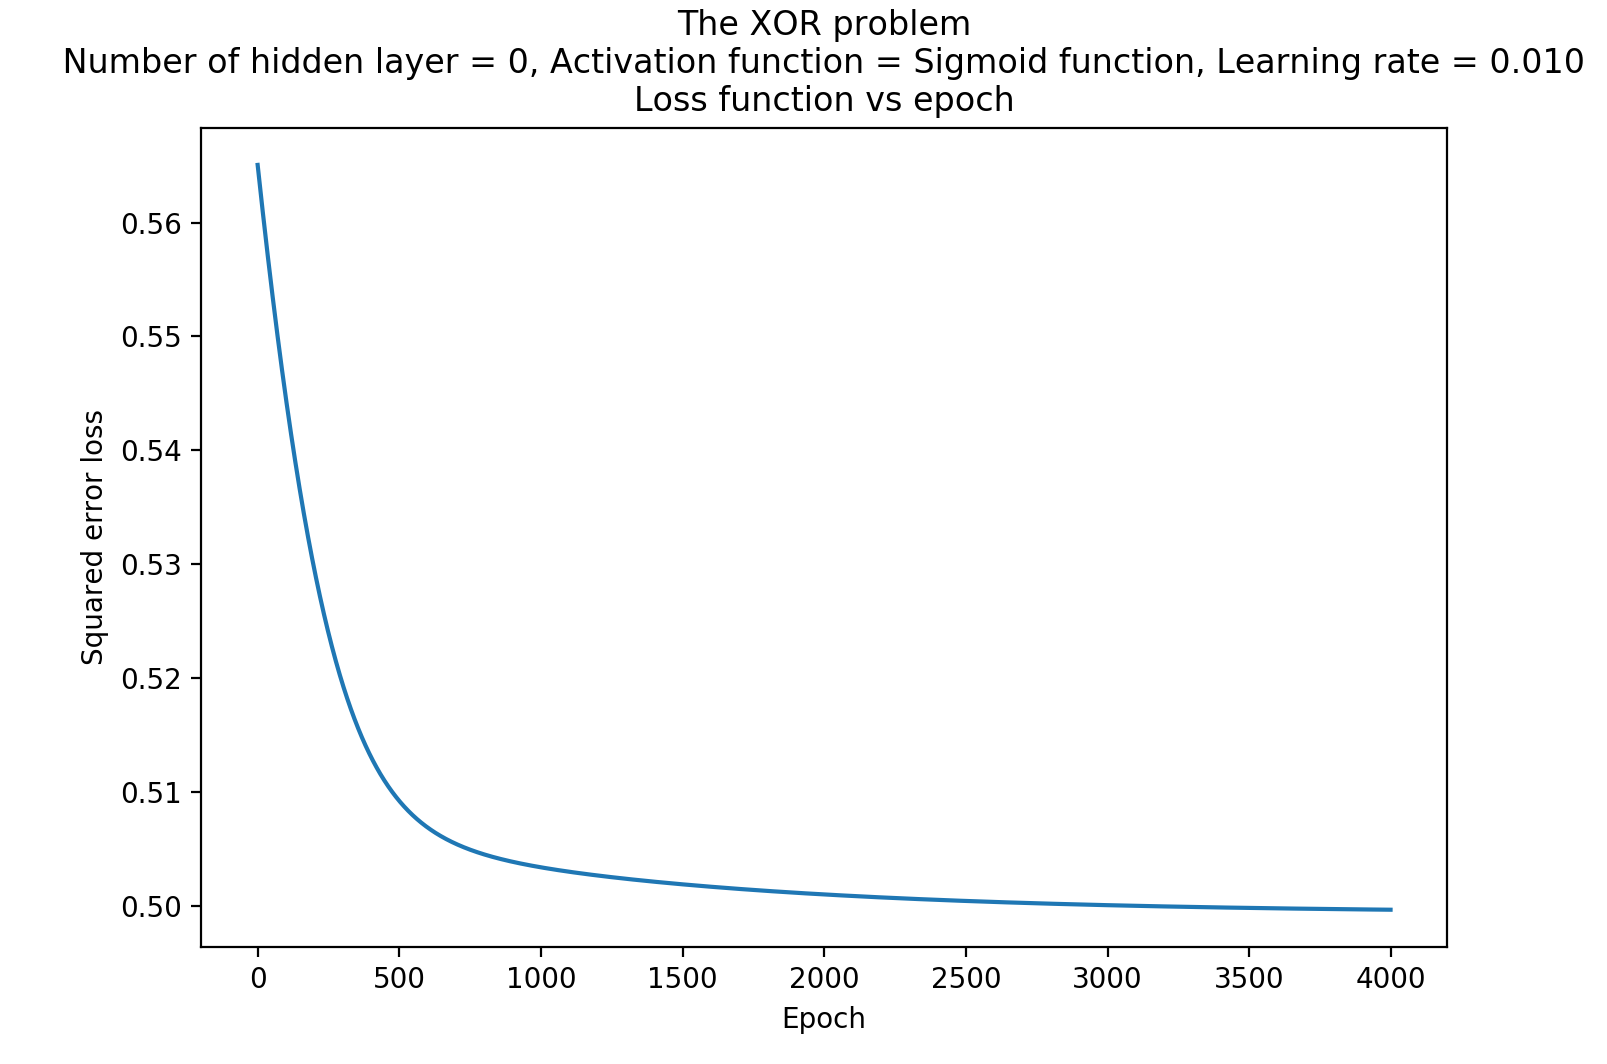
\includegraphics[width=0.49\columnwidth]{xor_sigmoid_mse_perceptron.png}
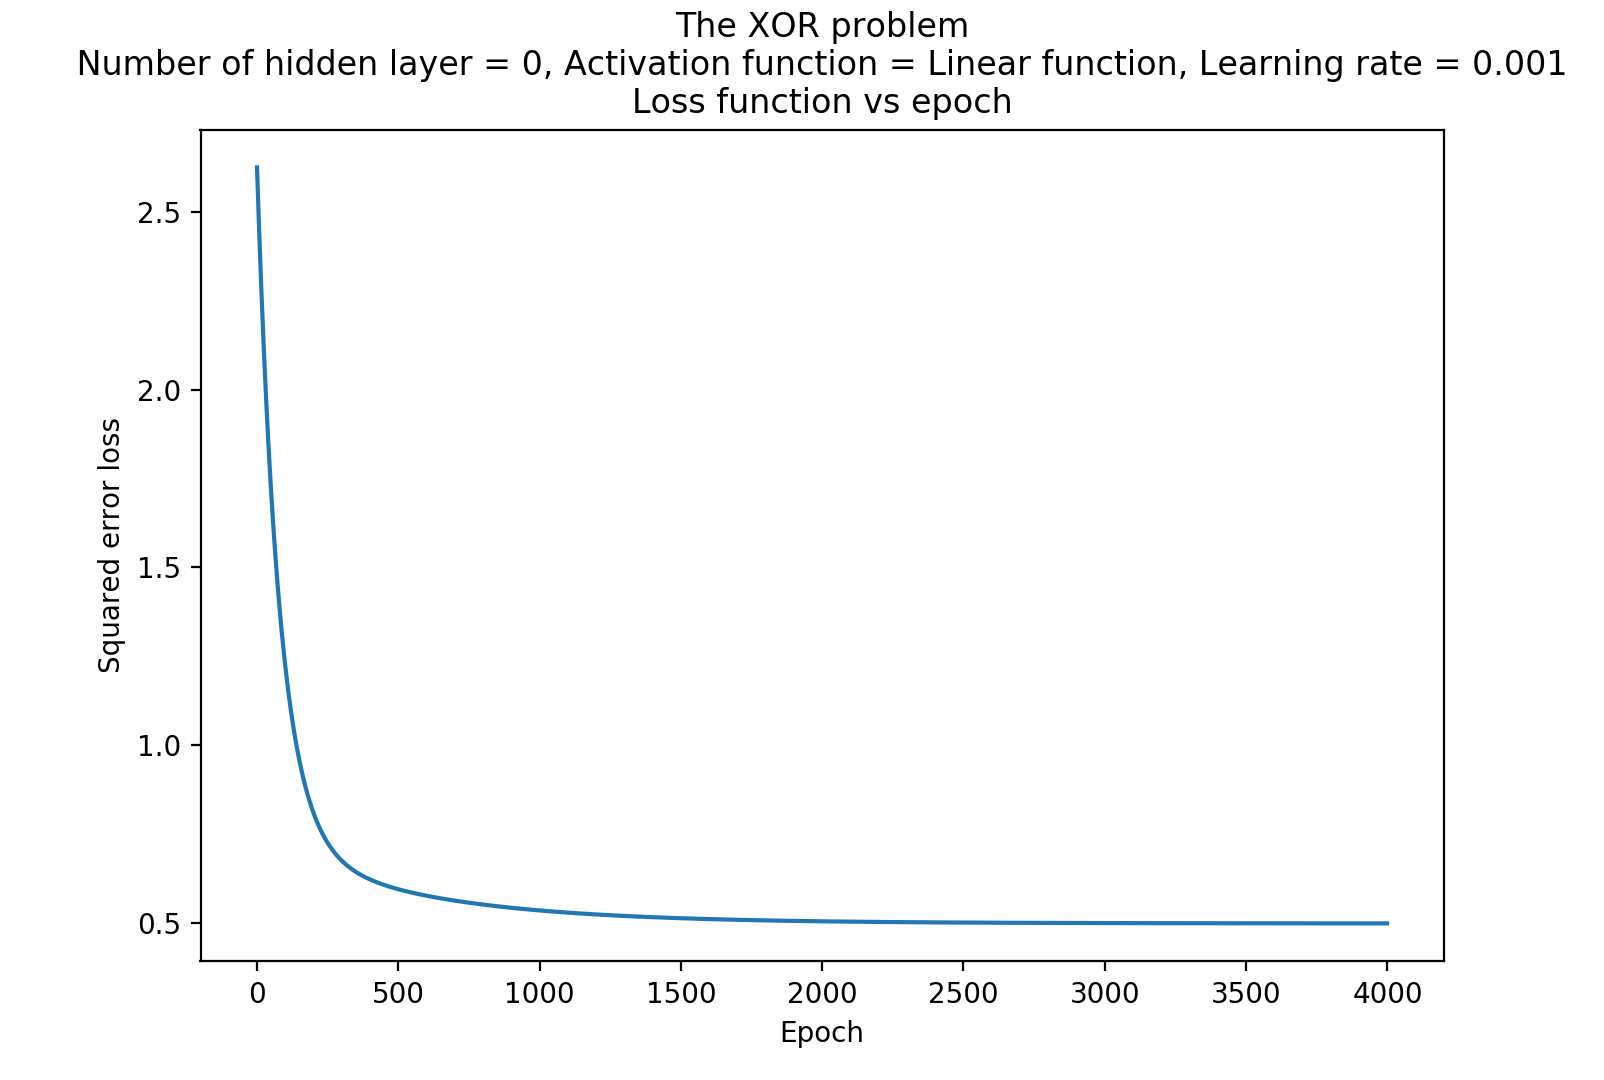
\includegraphics[width=0.49\columnwidth]{xor_linear_mse_perceptron.png}
\end{figure}

Single perceptron is unable to solve the XOR problem because XOR is a non-linear problem and single-layer perceptron is a linear approximator. \\

\pagebreak
\begin{multicols}{2}
Number of hidden layer: 1 \\
Activation function: Sigmoid \\
Loss function: Squared error\\
Learning rate: 5 \\
Number of iteration: 1000 \\
Predicted: $[[0.007], [0.992], [0.992], [0.010]]$ \\
Actual output: $[[0],[1],[1],[0]]$

Number of hidden layer: 1 \\
Activation function: Sigmoid \\
Loss function: Binary cross entropy\\
Learning rate: 2 \\
Number of iteration: 1000 \\
Predicted: $ [[0.000], [0.9997], [0.999], [0.000]]$ \\
Actual output: $[[0],[1],[1],[0]]$
\end{multicols}

\begin{figure}[h]
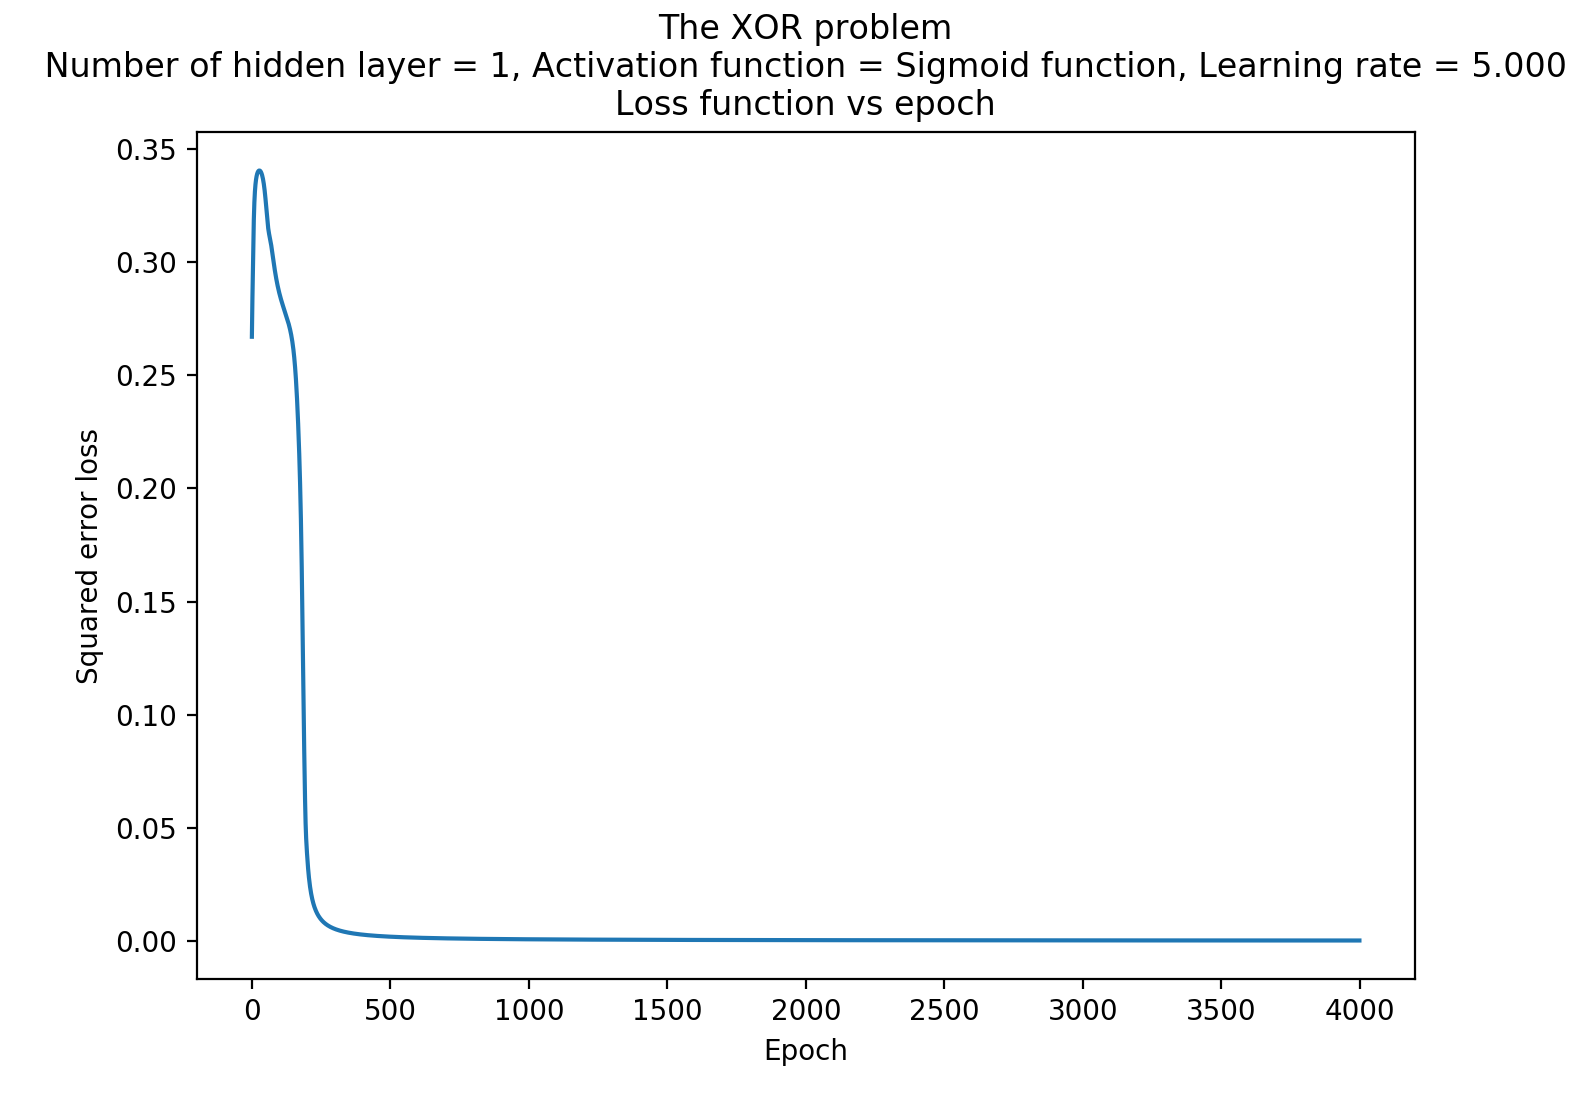
\includegraphics[width=0.49\columnwidth]{xor_sigmoid_mse.png}
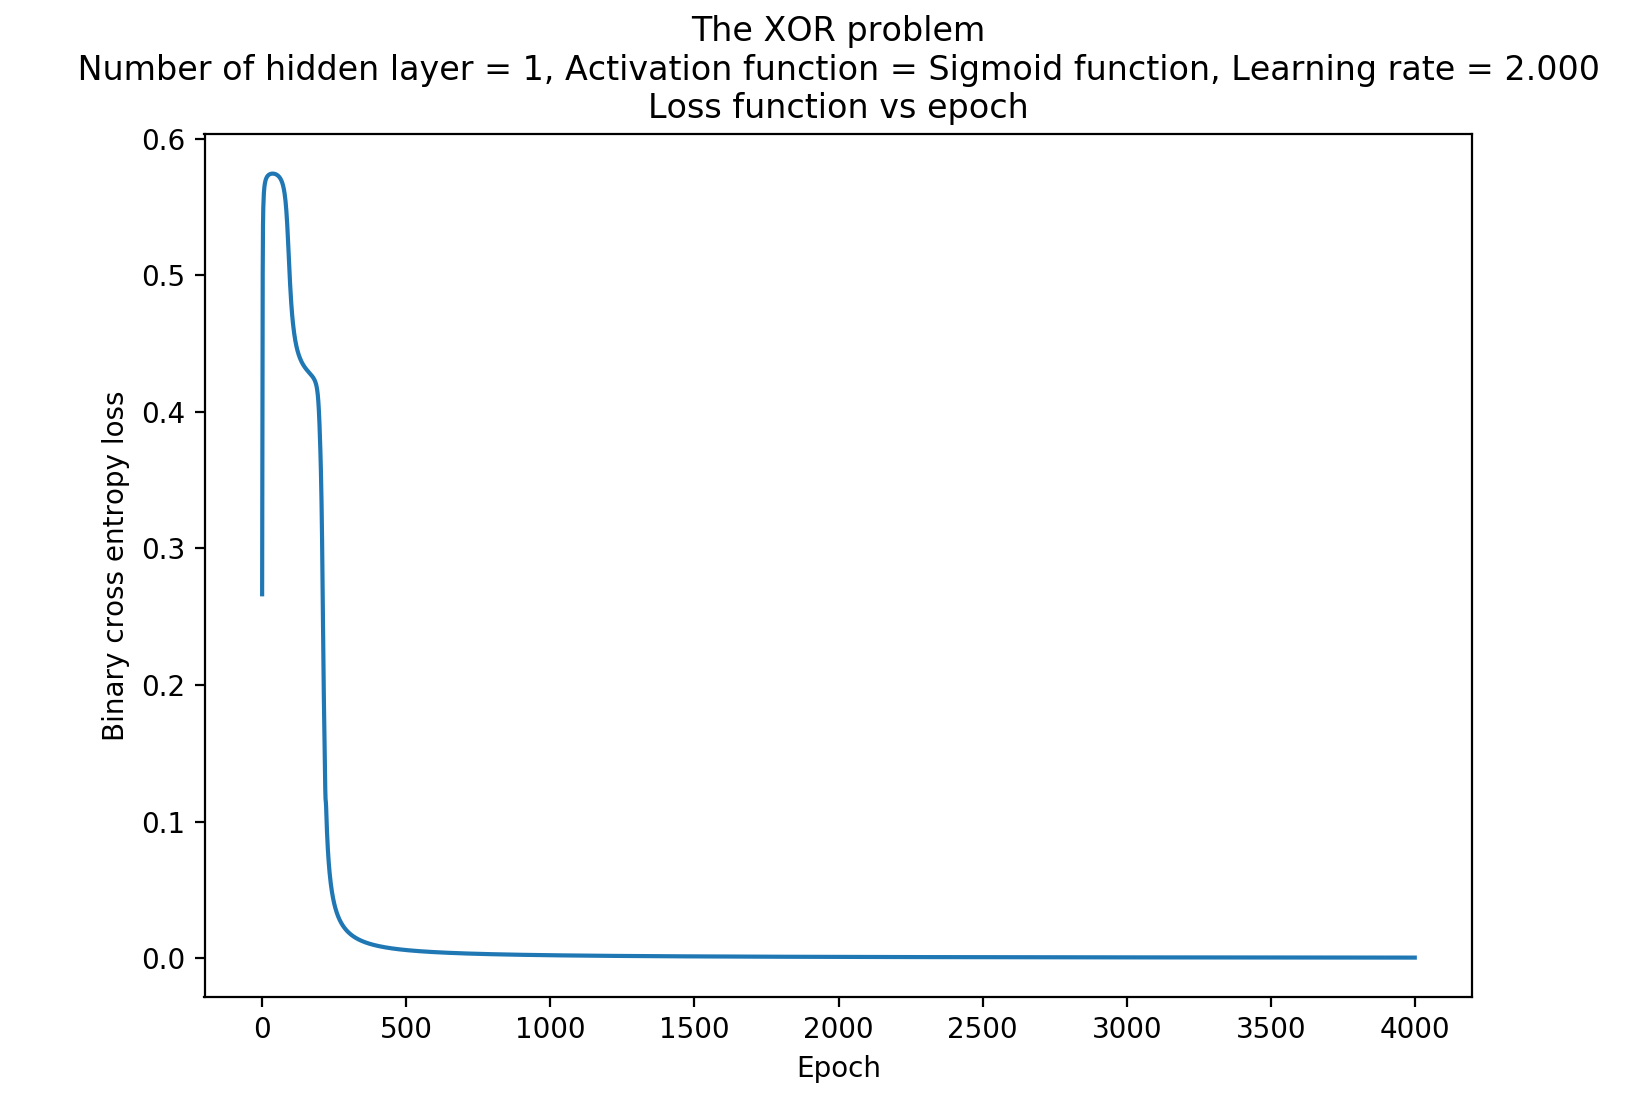
\includegraphics[width=0.49\columnwidth]{xor_sigmoid_bce.png}
\end{figure}

Using a sigmoid activation function on neural network with one hidden layer is able to solve the XOR problem because the neural network becomes a nonlinear approximator. \\

Number of hidden layer: 1 \\
Activation function: Linear \\
Loss function: Squared error\\
Learning rate: 5
Number of iteration: 1000 \\
Predicted: $[[0.417], [0.462], [0.528], [0.571]]$ \\
Actual output: $[[0],[1],[1],[0]]$ \\

\begin{figure}[h]
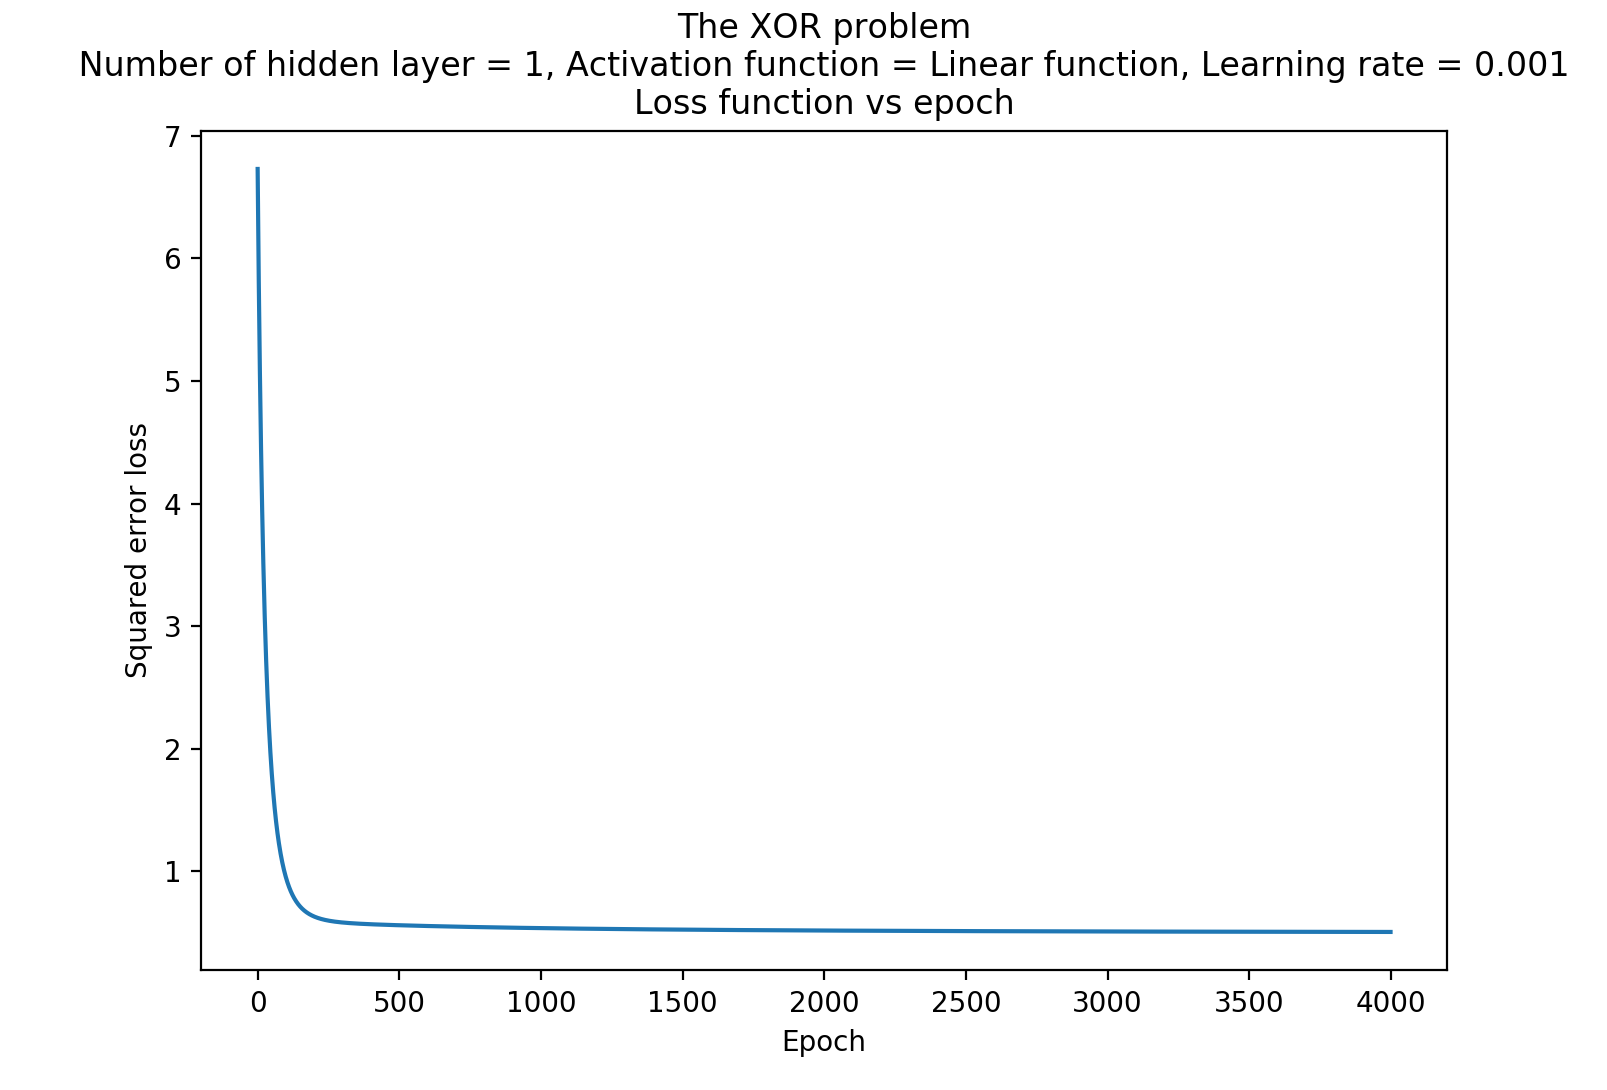
\includegraphics[width=0.49\columnwidth, left]{xor_linear_mse.png}
\end{figure}

Using linear activation function on multi-layer neural network essentially makes the neural network to be a linear approximator. Since XOR is a non-linear problem, this neural network is unable to solve the problem.


\pagebreak
\textbf{Single perceptron: loss functions vs epoch for different learning rates}

\begin{figure}[h]
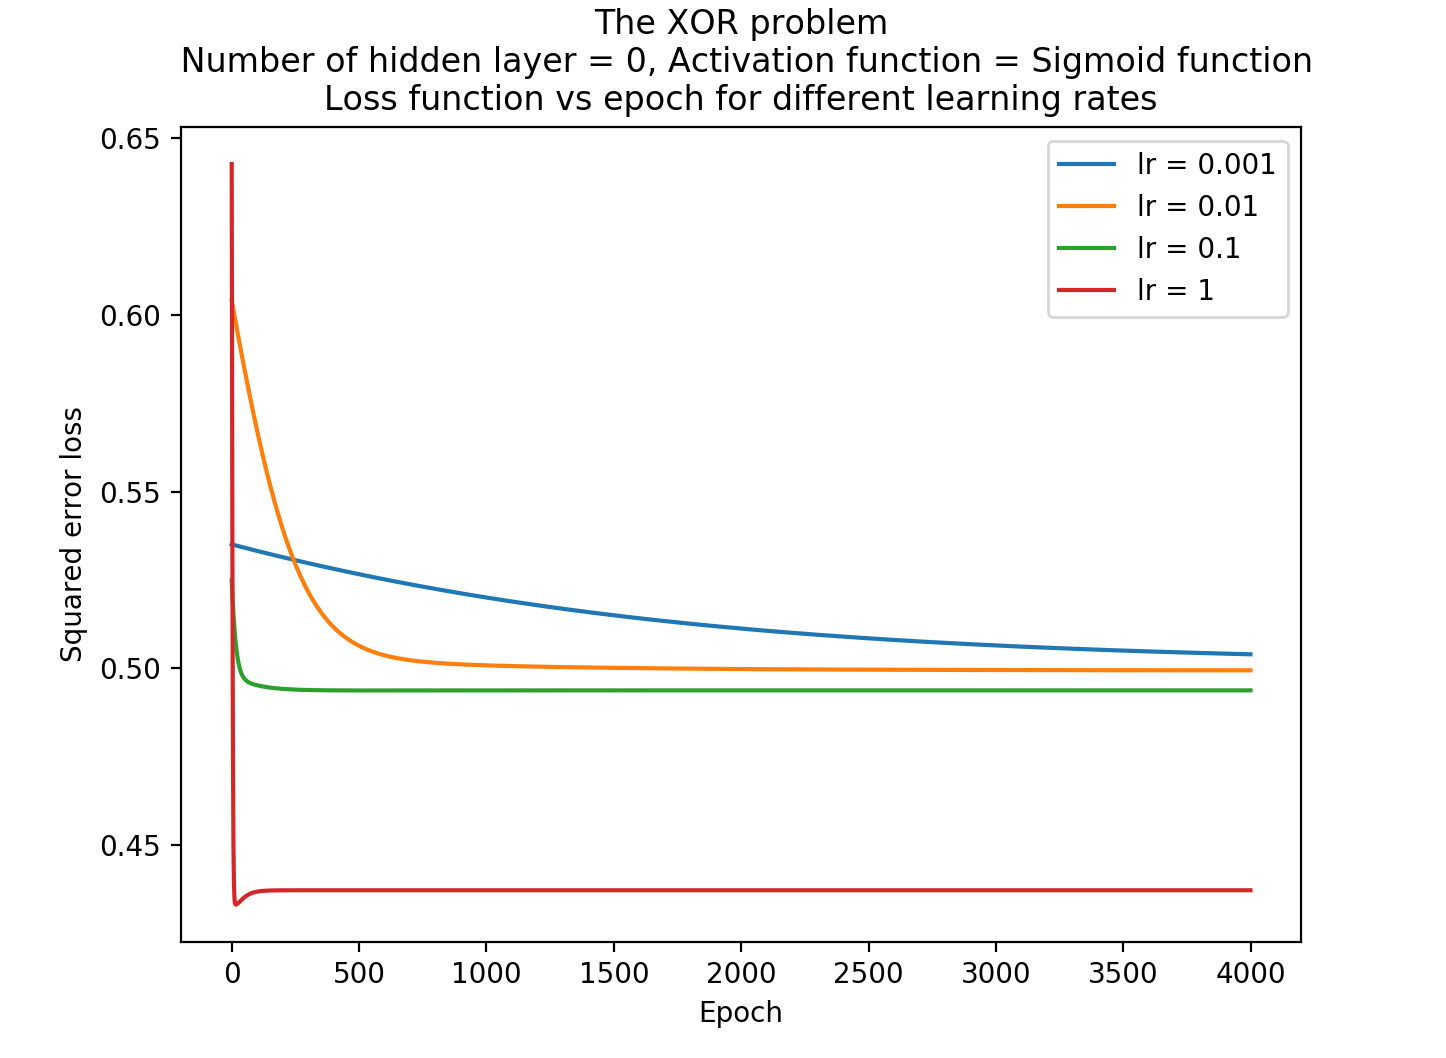
\includegraphics[width=0.49\columnwidth]{xor_sigmoid_mse_lrs_perceptron.png}
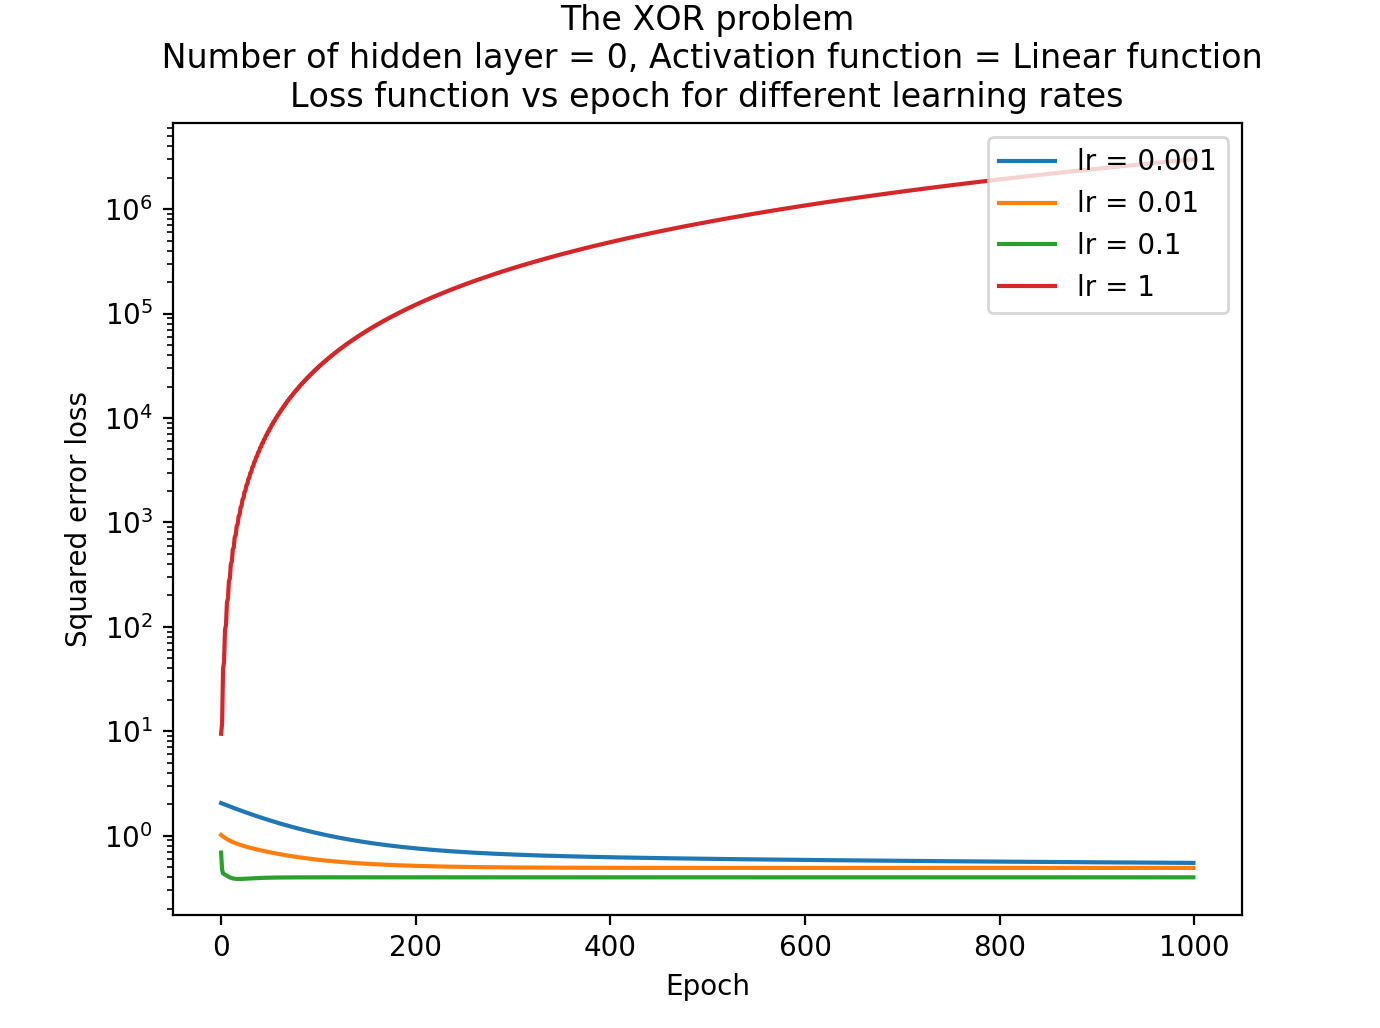
\includegraphics[width=0.49\columnwidth]{xor_linear_mse_lrs_perceptron.png}
\end{figure}

For sigmoid activation function, a larger learning rate seems to converge faster and has a lower loss. However, the overall loss is still larger than that of a hidden layer neural network. For linear activation function, too large of a learning rate results in an increasing loss. \\

\textbf{One hidden layer neural network: loss functions vs epoch for different learning rates}
\begin{figure}[h]
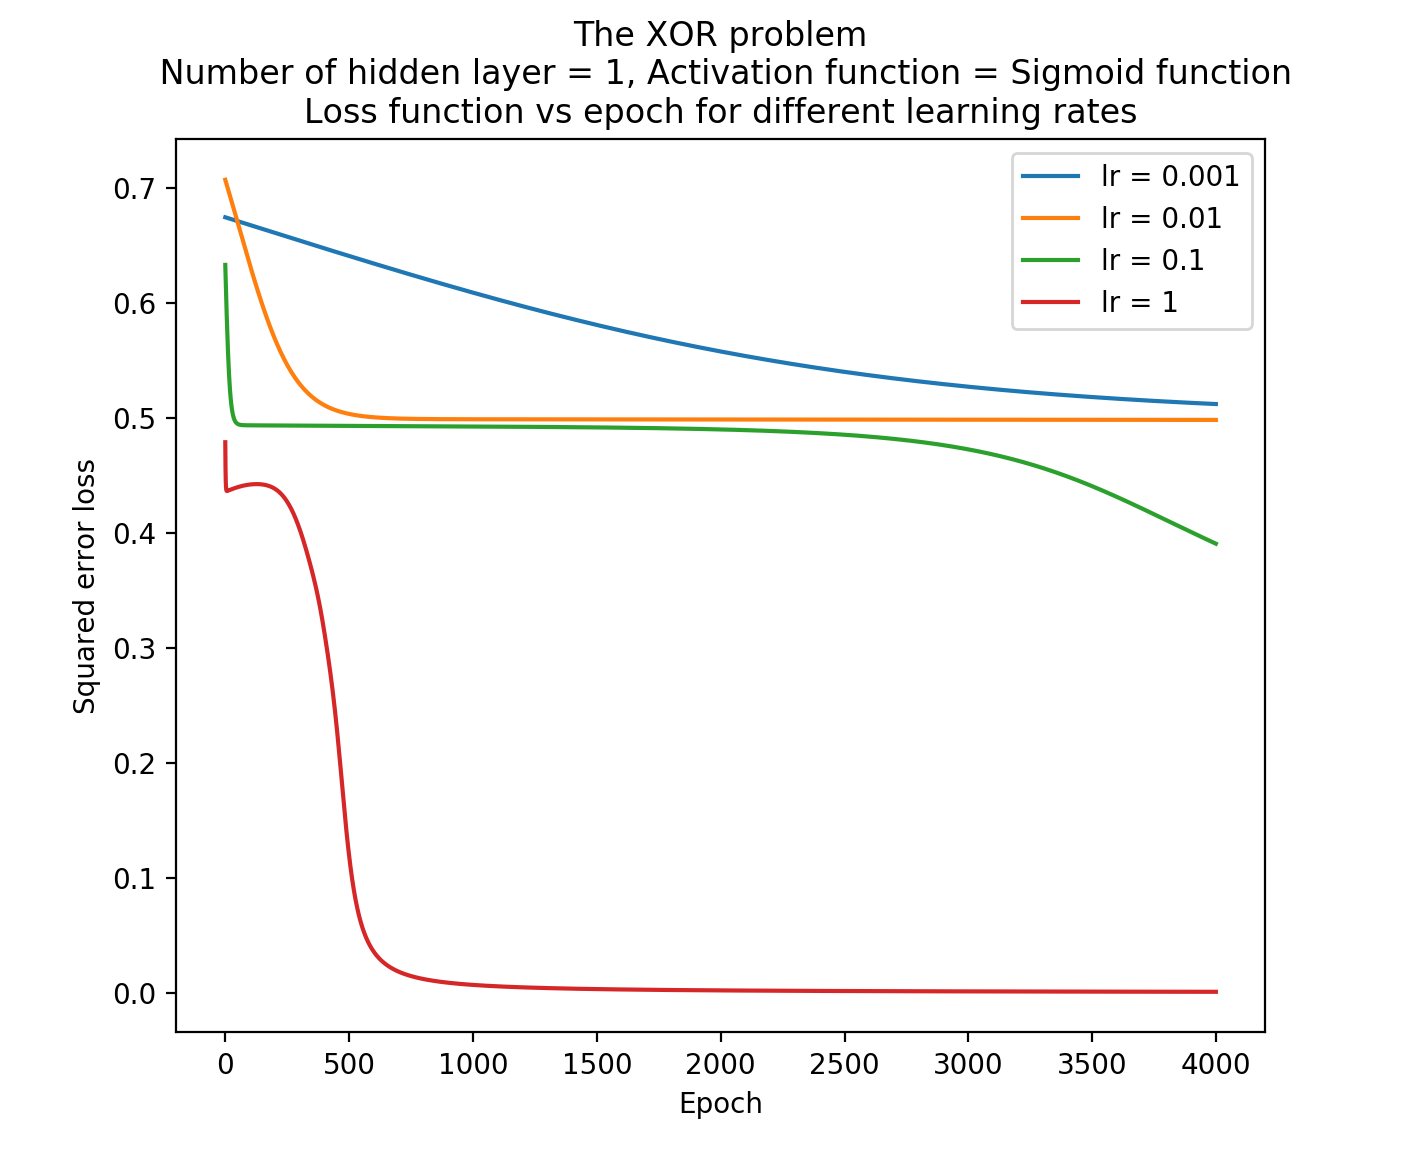
\includegraphics[width=0.49\columnwidth]{xor_sigmoid_mse_lrs}
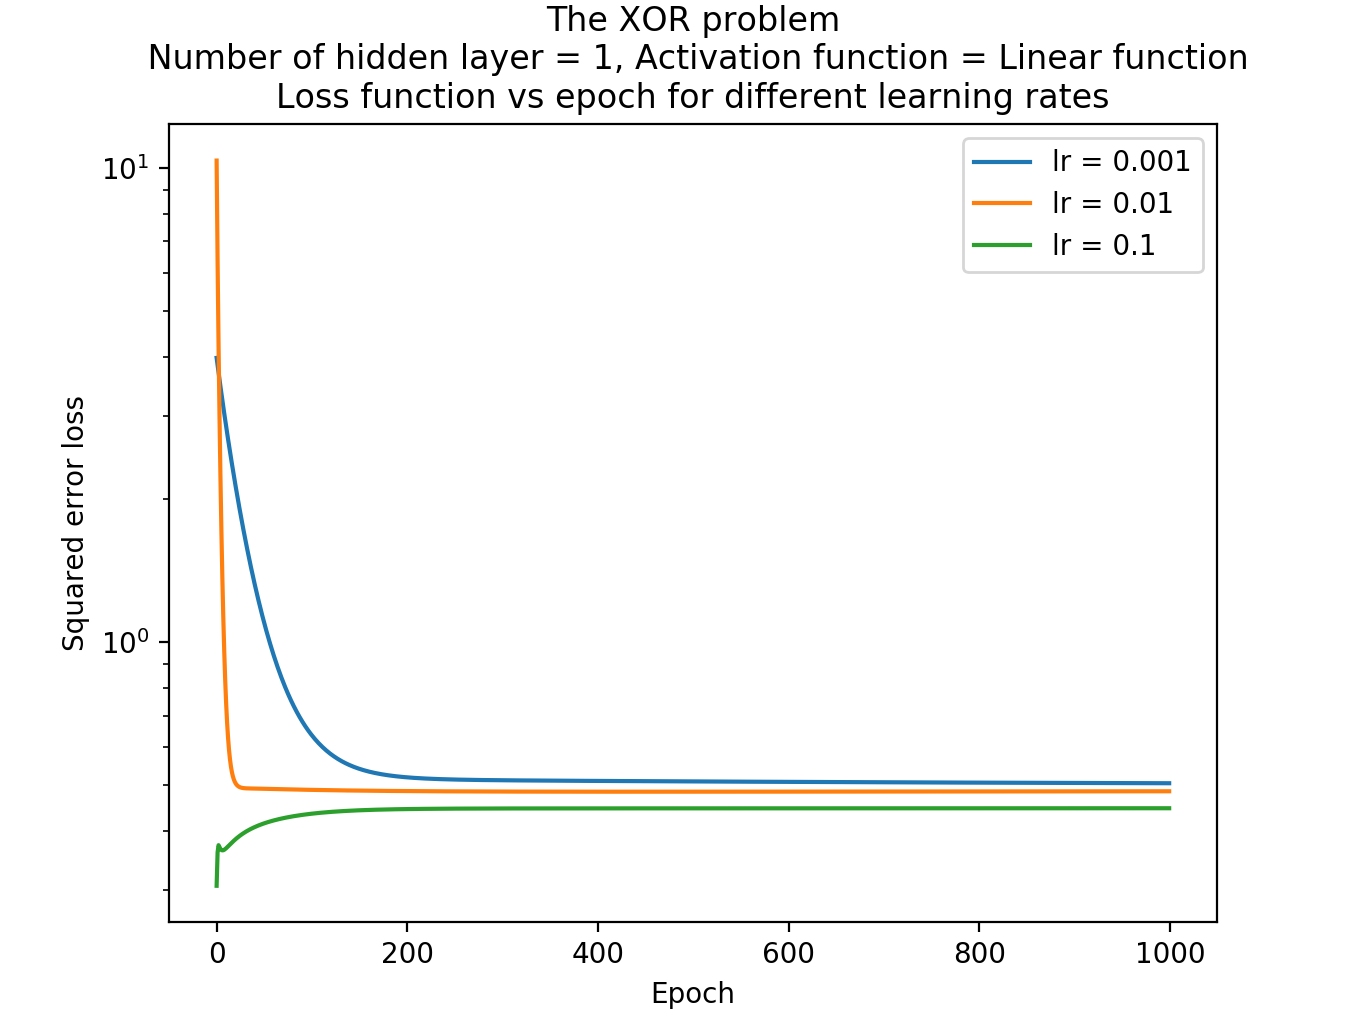
\includegraphics[width=0.49\columnwidth]{xor_linear_mse_lrs}
\end{figure}

For sigmoid activation function, a larger learning rate seems to converge faster and has a lower loss. For linear activation function, too large of a learning rate results in an increasing loss. \\


% \pagebreak

\end{document}